Hicimos el filtro {\ttfamily diff} tanto en C como en ASM. Su
implementación es bastante inmediata, al menos sin tener en cuenta los
registros {\ttfamily XMM} de {\ttfamily SSE}. De esta manera, el
filtro {\ttfamily diff} recorre todos los píxeles de ambas imágenes,
de forma secuencial, resta los tres componentes de colores y toma el
valor absoluto. Así, en cada píxel $(i, j)$ [de 4 bytes cada uno],
obtenemos tres bytes $(\Delta R, \Delta G, \Delta B)$. En este filtro
{\ttfamily diff}, convenimos que la imagen diferencia fuera la norma
infinito del vector en las tres posiciones (es decir, el máximo entre
los tres). Así, una vez obtenidos $(\Delta R, \Delta G, \Delta B)$,
calculamos el máximo entre los tres, $\Delta C$, y en el píxel
$(i, j)$ de la imagen de salida anotamos los tres bytes
$(\Delta C, \Delta C, \Delta C)$ y 0xFF en el canal
alpha. Repetimos este procedimiento para todos los píxeles de la
imagen.

En la implementación de ASM, aprovechamos los registros {\ttfamily
  SSE} disponibles en el procesador\footnote{El procesador utilizado,
  intel i7, tiene disponible {\ttfamily AVX}, pero no utilizamos estas
  instrucciones}. En cada registro entran 16 bytes: 4 píxeles que
pueden procesarse a la vez. Ahora procesarlos no es tan trivial como
antes, pero podemos ver que pensar algunas relaciones básicas de
álgebra, ayuda a ver el camino a seguir. Recordemos los dos pasos:

\paragraph{Restar los tres componentes y tomar valor absoluto} La clave
para reducir este problema es considerando la siguiente igualdad:

\begin{equation}
  \text{abs}(a - b) = \text{máx}(a, b) - \text{mín}(a, b)
\end{equation}

Así, simplemente tenemos que asegurarnos de estar restando el máximo
(byte a byte) menos el mínimo. Para eso, supongamos que tenemos las
tiras de 16 bytes de ambas imágenes en {\ttfamily XMM0} y {\ttfamily
  XMM3}. Ahora, copiamos cualquiera de los dos (por caso, {\ttfamily
  XMM0}) a un registro extra {\ttfamily XMM1}, y guardamos
{\ttfamily máx (XMM0, XMM3)} en {\ttfamily XMM0} [{\ttfamily
  pmaxub}]. Luego, guardamos {\ttfamily mín (XMM1, XMM3)} en
{\ttfamily XMM1} [{\ttfamily pminub}]. Ahora, {\ttfamily XMM0} tiene
los máximos y {\ttfamily XMM1} los mínimos, byte a byte, de los 4
píxeles. Los restamos byte a byte y guardamos el resultado en
{\ttfamily XMM0} [{\ttfamily psubb}]. Hacemos aquí unas cuentas
extras, ya que también estamos procesando el canal alpha. Esto no
significa un detrimento en performance (ya que la operación está
paralelizada), sino que si la información estuviera guardada en RGB
sin canal alpha se podrían procesar más píxeles a la
vez\footnote{Claro que ahora no podríamos garantizarnos esta
  hermosura de que entren \emph{justo} 4 píxeles en un registro
  {\ttfamily SSE}}.

\paragraph{Obtener el máximo} Ahora el desafío es encontrar, con
operaciones {\ttfamily SSE}, una forma de encontrar el máximo de
cada bloque de 4 bytes. Pensemos cada bloque de 4 bytes por separado
primero. Tenemos tres valores R, G, B, A y queremos que esto se
transforme en C, C, C, X [C es el máx(R, G, B) y X es el canal
alpha, que por ahora puede tomar cualquier valor]. Si $\mathbf{t}$
es el vector de salida, queremos
\begin{equation}
  \mathbf{t} = (\text{máx}(R, G, B), \text{máx}(R, G, B), \text{máx}(R, G, B))
\end{equation}

Para vectorizar esta expresión, tenemos que usar la siguiente identidad:

\begin{equation}
  \text{máx}(R, G, B) = \text{máx}(R, \text{máx}(G, B)) =
  \text{máx}(G, \text{máx}(B, R)) = \text{máx}(B, \text{máx}(R, G))
  \label{eq:max_circ}
\end{equation}

Definimos al vector $\mathbf{p} = (R, G, B)$ y al operador
{\ttfamily rot} tal que:

\begin{equation}
  \text{rot}(R, G, B) = (G, B, R) 
\end{equation}

Las sucesivas aplicaciones de {\ttfamily rot} las definimos también: 

\begin{align}
  \mathbf{q} &= \text{rot}(R, G, B) = (G, B, R) \\
  \mathbf{r} &= \text{rot}(\text{rot}(R, G, B)) = (B, R, G)
\end{align}

Con esta notación, la identidad~\ref{eq:max_circ} queda

\begin{equation}
  \text{máx}(R, G, B) = \text{máx}(p_1 \text{máx}(q_1, r_1)) =
  \text{máx}(p_2, \text{máx}(q_2, r_2)) = \text{máx}(p_3, \text{máx}(q_3, r_3))
\end{equation}

y, en consecuencia, $\mathbf{t}$ es

\begin{equation}
  \mathbf{t} = \text{máx}(\mathbf{p}, \text{máx}(\mathbf{q}, \mathbf{r}))
\end{equation}

Esta ecuación ahora está vectorizada y podemos usar {\ttfamily
  pmaxub} para calcular los máximos Sólo queda crear, a partir de
$\mathbf{p}$ los vectores rotados $\mathbf{q}$ y $\mathbf{r}$; es
decir, implementar el operador {\ttfamily rot}. Para esto,
utilizamos una máscara que rota a la izquierda los tres bytes, es
decir: $(R, G, B) \rightarrow (G, B, R)$, utilizando {\ttfamily
  pshufb} y una máscara del tipo (1, 2, 0).

Como, en rigor, en cada píxel tenemos también el canal alpha, la
máscara para cada byte va a ser (1, 2, 0, 0xFF), poniendo un 0 en el
canal alpha [esto también podría ser la posición 3 o cualquier otra,
porque el canal alpha \emph{tiene que} ser reescrito].


Esto explica el procedimiento general. Aumentarlo para procesar $n$
píxeles en paralelo es directo, simplemente la máscara de rotación
va a ser
$\mathbf{m} = (1, 2, 0, \text{0xFF}, 4+1, 4+2, 4+0, \text{0xFF}, 8+1, 8+2, 8+0,
\text{0xFF}, \ldots)$. En general, 

\begin{equation}
  m_i = \left\{
    \begin{array}{ll}
      4*\text{floor}(i/4) + \text{mod}(i + 1, 3) & \quad \text{mod}(i, 4) \ne 3 \\
      \text{0xFF} & \quad \text{mod}(i, 4) = 3
    \end{array}
  \right.
\end{equation}

La implementación entonces es directamente una traducción de esto:
Copiamos el registro {\ttfamily XMM0} ($\mathbf{p}$) a un registro
{\ttfamily XMM1} y mantenemos la máscara de rotación en {\ttfamily
  XMM2}. Ahora rotamos {\ttfamily XMM1} con {\ttfamily pshufb} y
obtenemos $\mathbf{q}$. Obtenemos el máximo de {\ttfamily XMM0}
($\mathbf{p}$) y {\ttfamily XMM1} ($\mathbf{q}$) con {\ttfamily
  pmaxub} y lo guardamos en {\ttfamily XMM0}. Rotamos nuevamente
{\ttfamily XMM1} y resulta $\mathbf{r}$. Ahora calculamos el máximo
de {\ttfamily XMM0} ($\text{máx}(\mathbf{p}, \mathbf{q})$) y
{\ttfamily XMM1} ($\mathbf{r}$) y lo guardamos en {\ttfamily XMM0}
(el objetivo final, $\mathbf{t}$).

En la figura~\ref{fig:esquema_diff} se puede observar un esquema de este
procedimiento.


\begin{figure}
  \centering
  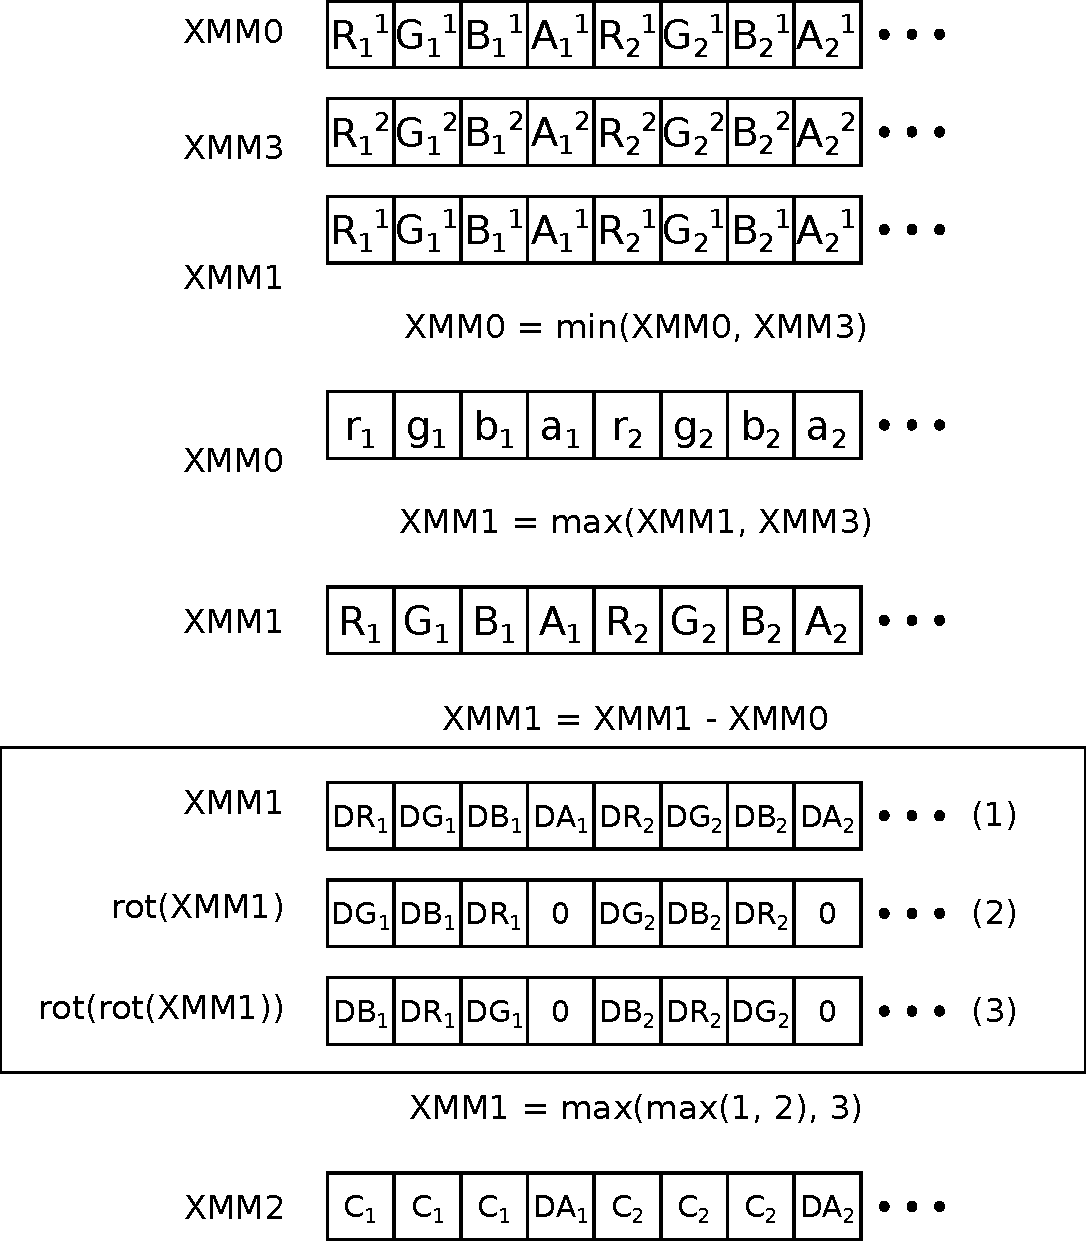
\includegraphics[width=0.7\columnwidth]{esquema_diff.pdf}
  \caption{Esquema que caracteriza el algoritmo de diff con
    instrucciones {\ttfamily SIMD}}
  \label{fig:esquema_diff}
\end{figure}


\subsubsection{Iteración del Ciclo Principal}

Vamos a mostrar como se cargan y modifican los registros en una iteración de nuestra implementación

\subsubsection{Sección .data}

\indent Definimos una constantes en la sección .data (por ende es una constantes inicializada) 
\begin{itemize}

\item mask\char`_rot: DB 1, 2, 0, 0xFF, 5, 6, 4, 0xFF, 9, 10, 8, 0xFF, 13, 14, 12, 0xFF : es una máscara que utilizaremos para acomodar los canales

\end{itemize}


\subsubsection{Carga de datos}


\indent La carga de datos inicial para el ciclo principal del algoritmo es:


\begin{itemize}
\item Copiamos en {\ttfamily XMM2} la m\'ascara mask\char`_rot
\item Inicializamos {\ttfamily R9} en 0 con la instrucción {\ttfamily XOR} para utilizarlo de contador de columnas
\item Inicializamos {\ttfamily R10} en 0 con la instrucción {\ttfamily XOR} para utilizarlo de contador de filas
\item Preservamos en {\ttfamily R8} m y lo usamos para saber cu\'ando terminamos una columna
\item Preservamos en {\ttfamily RCX} n y lo usamos para saber cu\'ando terminamos una fila

\end{itemize}

\subsubsection{Ciclo Principal}


\indent Con los datos cargados en los registros vamos a mostrar una iteraci\'on del ciclo principal del filtro. Para cada l\'inea de la matriz que representa la imagen fuente se realizan las siguientes acciones.

\begin{itemize}
\item Leemos desde la primer imagen fuente en {\ttfamily RDI} 16 bytes y los cargamos en {\ttfamily XMM0}, cargando aqui la fila $i - 1$ con la instrucción {\ttfamily MOVDQU}
\item Leemos desde la segunda imagen fuente en {\ttfamily RSI} 16 bytes y los cargamos en {\ttfamily XMM3}, cargando aqui la fila $i - 1$ con la instrucción {\ttfamily MOVDQU}

\item Obteniendo en cada uno de los registros

\begin{center}
\xmmxByteHighBig{$A2$}{$B2$}{$G2$}{$R2$}{$A3$}{$B3$}{$G3$}{$R3$}\xmmxByteLowBig{$A0$}{$B0$}{$G0$}{$R0$}{$A1$}{$B1$}{$G1$}{$R1$}
\end{center}


\end{itemize}
